% Task 6: a cheap generator. Ciphertext from Task6/cheap.py (32 bytes);
% CHECKED (python3): 0xF3 XOR 'D' (0x44) = 0xB7 = k1. k2, k3, k4 and the message are the result of the task: not shown.
%   The good generator row is the RC4 keystream of the key "Kangaroo" (Task 2): 69 9d da 7e fe 61 73 62 97 c5 8c ab
\documentclass[12pt,tikz,border=6pt]{standalone}
% Shared preamble of the task figures of Lecture 1.
% The colours and styles are copied from the preamble of ../main.tex (keep them in sync).
\usepackage{lmodern}
\usepackage[T1]{fontenc}
\renewcommand{\familydefault}{\sfdefault}
\usepackage{amsmath,amssymb}
\usepackage{xcolor}
\usepackage{fontawesome5}
\usetikzlibrary{arrows.meta, calc, positioning, fit, decorations.pathreplacing, decorations.pathmorphing, backgrounds}

% ---------- template ----------
\definecolor{DeepBlue}{HTML}{283593}
\definecolor{AccentOrange}{HTML}{EB5A14}
\definecolor{LightGray}{HTML}{F5F6FA}
% ---------- actors and categories (S1 to S6) ----------
\definecolor{sIndigo}{HTML}{5C6BC0}   % the sender
\definecolor{sPink}{HTML}{EC407A}     % the attacker
\definecolor{sViolet}{HTML}{7E57C2}   % plaintext
\definecolor{sAmber}{HTML}{FFB300}    % key and keystream
\definecolor{sTeal}{HTML}{26A69A}     % the receiver
\definecolor{sBrown}{HTML}{8D6E63}    % ciphertext
\definecolor{sPinkText}{HTML}{C2185B}
\definecolor{sAmberText}{HTML}{A06A00}
\definecolor{sTealText}{HTML}{00796B}
% ---------- actions and results ----------
\definecolor{aExec}{HTML}{43A047}
\definecolor{aRead}{HTML}{1E88E5}
\definecolor{aWrite}{HTML}{E53935}
% ---------- neutral ----------
\definecolor{nInk}{HTML}{37474F}
\definecolor{nLine}{HTML}{90A4AE}
\definecolor{nLight}{HTML}{CFD8DC}
\definecolor{nFill}{HTML}{ECEFF1}
\definecolor{nIdle}{HTML}{E0E0E0}

% ---------- TikZ styles (as in main.tex; byte cells a little larger for the web) ----------
\tikzset{
  hw/.style={draw=nLine, thick, fill=nFill, text=nInk, rounded corners=3pt, align=center, inner sep=4pt},
  hwmain/.style={draw=nInk, thick, fill=nInk, text=white, rounded corners=3pt, align=center, inner sep=4pt},
  cell/.style={draw=nLine, thick, fill=white, text=nInk, font=\ttfamily\small},
  cellfree/.style={cell, dashed, draw=nLight},
  container/.style={draw=nLine, thick, dashed, rounded corners=5pt},
  actor/.style={fill=#1, draw=#1, text=white, rounded corners=3pt, align=center, font=\small\bfseries, inner sep=5pt},
  actorlight/.style={fill=#1!15, draw=#1, thick, text=nInk, rounded corners=3pt, align=center, inner sep=5pt},
  data/.style={-{Stealth}, very thick, nInk},
  flow/.style={-{Stealth}, very thick, DeepBlue},
  annot/.style={draw=AccentOrange, line width=1.6pt, rounded corners=3pt},
  byte/.style={draw=nLine, thick, fill=white, text=nInk, font=\ttfamily\small,
    minimum width=0.8cm, minimum height=0.62cm, inner sep=1pt, rounded corners=1.5pt},
  ptb/.style={byte, fill=sViolet!15, draw=sViolet},
  ksb/.style={byte, fill=sAmber!25, draw=sAmber},
  ctb/.style={byte, fill=sBrown!15, draw=sBrown},
  unk/.style={byte, fill=white, dashed, text=sViolet},
  rowlabel/.style={font=\small\bfseries, text=nInk, anchor=east},
  note/.style={font=\small, text=nInk},
  bigxor/.style={circle, draw=nInk, very thick, fill=white, inner sep=0pt, minimum size=0.8cm, font=\Large},
  radio/.style={-{Stealth}, very thick, nInk, decorate,
    decoration={snake, amplitude=1.2pt, segment length=7pt, post length=4pt}},
  % a white card behind the whole figure, so that it stays readable in a dark theme
  card/.style={show background rectangle, background rectangle/.style={fill=white, draw=none}, inner frame sep=8pt},
}
% a row of bytes: \byterow{x of the first cell}{y}{style}{list of values}{step between cells}
\newcommand{\byterow}[5]{%
  \expandafter\def\expandafter\brlist\expandafter{#4}%
  \foreach \v [count=\k from 0] in \brlist {
    \node[#3] at ({#1+#5*\k},#2) {\v};
  }}
% the generator / cipher box: dark, with cogs. \cogbox{name}{position}{label}{width}
\newcommand{\cogbox}[4]{%
  \node[hwmain, minimum width=#4, minimum height=1.3cm] (#1) at (#2) {};
  \node[text=white, font=\Large] at ([yshift=0.22cm]#1.center) {\faCogs};
  \node[text=white, font=\small\bfseries] at ([yshift=-0.32cm]#1.center) {#3};}
\newcommand{\ok}{\textcolor{aExec}{\faCheck}}
\newcommand{\nok}{\textcolor{aWrite}{\faTimes}}
\newcommand{\badge}[1]{\tikz[baseline=(b.base)]\node[circle,fill=AccentOrange,text=white,
  inner sep=1.5pt,font=\bfseries\footnotesize] (b) {#1};}

\begin{document}
\pagecolor{white}
\begin{tikzpicture}[>=Stealth]
  \def\dx{1.0}
  \def\xs{4.6}
  % the four keystream numbers: four shades of the keystream colour
  \tikzset{
    k1/.style={byte, draw=sAmber, fill=sAmber!75, font=\small\bfseries},
    k2/.style={byte, draw=sAmber, fill=sAmber!45, font=\small\bfseries},
    k3/.style={byte, draw=sAmber, fill=sAmber!20, font=\small\bfseries},
    k4/.style={byte, draw=sAmber, fill=white, font=\small\bfseries},
  }
  \newcommand{\krow}[1]{\foreach \k in {0,...,11} {\pgfmathtruncatemacro{\m}{mod(\k,4)+1}\node[k\m] at ({\xs+\dx*\k},#1) {k\m};}}

  % ---------- two generators ----------
  \node[hwmain, minimum width=3.6cm, minimum height=0.9cm, font=\small\bfseries] (g1) at (1.6,3.3) {\faCogs\ cheap generator};
  \draw[data] (g1.east) -- ({\xs-0.55},3.3);
  \krow{3.3}
  \node[text=nInk] at ({\xs+12*\dx-0.1},3.3) {\ldots};
  \foreach \s in {0,4,8} \draw[decorate, decoration={brace, amplitude=4pt}, nInk] ({\xs+\dx*\s-0.4},3.72) -- ({\xs+\dx*(\s+3)+0.4},3.72);
  \node[font=\small\bfseries, text=AccentOrange, anchor=west] at ({\xs+12.4*\dx},3.3) {repeats};
  \node[note] at ({\xs+5.5*\dx},4.2) {the same 4 numbers, again and again};

  \node[hwmain, minimum width=3.6cm, minimum height=0.9cm, font=\small\bfseries] (g2) at (1.6,2.0) {\faCogs\ RC4};
  \draw[data] (g2.east) -- ({\xs-0.55},2.0);
  \byterow{\xs}{2.0}{ksb}{69,9D,DA,7E,FE,61,73,62,97,C5,8C,AB}{\dx}
  \node[text=nInk] at ({\xs+12*\dx-0.1},2.0) {\ldots};
  \node[font=\small\bfseries, text=sTealText, anchor=west] at ({\xs+12.4*\dx},2.0) {does not repeat};

  \draw[nLight, thick, dashed] (-0.3,1.25) -- (18.3,1.25);

  % ---------- the message under the cheap generator ----------
  \node[rowlabel] at ({\xs-0.6},0.65) {position \texttt{i}};
  \foreach \k in {0,...,11} \node[font=\small, text=gray] at ({\xs+\dx*\k},0.65) {\k};
  \node[rowlabel] at ({\xs-0.6},0.15) {\texttt{i \% 4}};
  \foreach \k in {0,...,11} {\pgfmathtruncatemacro{\m}{mod(\k,4)}\node[font=\small\bfseries, text=nInk] at ({\xs+\dx*\k},0.15) {\m};}
  \node[rowlabel] at ({\xs-0.6},-0.5) {ciphertext};
  \byterow{\xs}{-0.5}{ctb}{F3,4F,84,12,97,68,8A,02,9B,0A,91,08}{\dx}
  \node[text=nInk] at ({\xs+12*\dx-0.1},-0.5) {\ldots};
  \node[rowlabel] at ({\xs-0.6},-1.3) {XOR keystream};
  \krow{-1.3}
  \node[text=nInk] at ({\xs+12*\dx-0.1},-1.3) {\ldots};
  \draw[nInk, thick] ({\xs-0.45},-1.75) -- ({\xs+11.45*\dx},-1.75);
  \node[rowlabel] at ({\xs-0.6},-2.2) {message};
  \byterow{\xs}{-2.2}{ptb, font=\ttfamily\normalsize\bfseries}{D,e,a,r}{\dx}
  \foreach \k in {4,...,11} \node[unk] at ({\xs+\dx*\k},-2.2) {?};
  \node[text=nInk] at ({\xs+12*\dx-0.1},-2.2) {\ldots};
  \node[font=\small, text=nInk, anchor=west] at ({\xs+12.4*\dx},-0.5) {32 bytes};
  % the known start gives the 4 numbers
  \draw[annot] ({\xs-0.5},-2.6) rectangle ({\xs+3.5*\dx},-0.1);
  \node[font=\small, text=AccentOrange, anchor=north west, align=left] at (-0.3,-2.75)
    {\textbf{Known start} \texttt{Dear} gives the 4 numbers. Example: \texttt{k1 = 0xF3 XOR \textquotesingle D\textquotesingle\ = 0xB7}.\\
     Then \texttt{k1} also opens bytes 4, 8, 12, \ldots, \texttt{k2} opens bytes 5, 9, 13, \ldots: the whole message.};
\end{tikzpicture}
\end{document}
